\index{Newton method}
\chapter{Newton Methods}
\printchapterversion{4_newton_methods}
\newthought{A Step in the Right direction.}

% TODO
% Think about introducing fixpoint iterations as a family first, then introduce Newton as a specific method within that family.

% TODO
% Introduce the convergence order of the Secant method: super-linear with
% p = phi = (1 + sqrt(5)) / 2 ~ 1.618 (the golden ratio). Sits between linear
% (e.g. bisection) and quadratic (Newton). Worth contrasting explicitly with
% Newton's p = 2, so students can reason about iteration counts to reach a
% given tolerance.



% ==============================================================================================
% INTRODUCTION BLOCK

\section{The Why}

\index{local information}
\index{derivative}
\newthought{In the previous chapter}, 
we characterized numerical methods with conditioning, stability, consistency, and convergence.
But our brute-force grid search is fundamentally limited: it explores the solution space blindly, 
requiring $O(N^d)$ evaluations for $N$ grid points in $d$ dimensions.

\newthought{The key insight} is deceptively simple: instead of asking "what is the value here?" at every grid point, we also ask "which way should I go next?".
The function's slope, its derivative, tells us the direction towards the solution.
This transforms search fundamentally.

\newthought{Understanding these methods} allows us to:
\begin{itemize}
    \item Use local information to make sophisticated steps instead of brute-force searches
    \item Achieve faster and more optimal convergence.
\end{itemize}

\index{gradient descent}
\newthought{In Machine Learning and Deep Learning,} Newton's method simplified to first order is also known as 
gradient descent. One could argue that the entire field of deep learning is built on the idea of using 
local gradient information to navigate toward minima in a high-dimensional loss landscape, 
to train models that are optimized towards specific objectives.

\marginnote{\newthought{Backpropagation} is of course as vital to distribute gradient information through the layers of a neural network, but the core optimization step is still a form of gradient-based navigation.}








\newpage
\subsection{Hands On Experience}

For starters let's get an intuitive feel for the power of using local information.
We compare grid search with Newton's method on the same sine function from Chapter 3, 
but now we're finding where it crosses zero: $\sin(x) = 0$ on the interval $[2.5, 4]$ 
(the solution is near $\pi \approx 3.14159$). 



\begin{figure}[h]
    \centering
    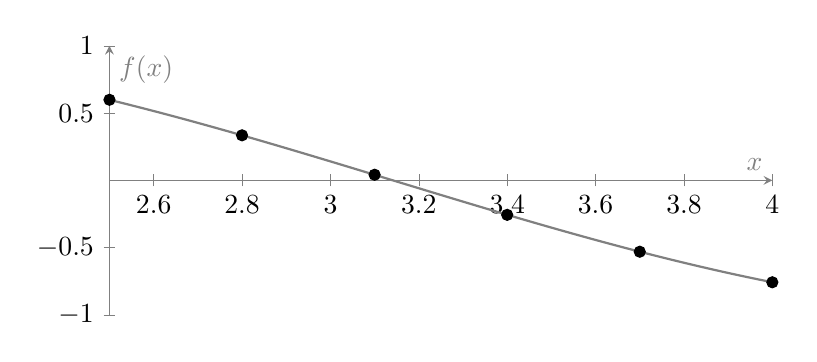
\begin{tikzpicture}
        \begin{axis}[
              width=10cm,
              height=5cm,
              axis x line=middle,
              axis y line=middle,
              xlabel={$x$},
              ylabel={$f(x)$},
              domain=2.5:4,
              samples=100,
              ymin=-1, ymax=1,
              xmin=2.5, xmax=4,
              legend style={at={(0.5,-0.2)},anchor=north},
              tick style={gray},
              label style={gray},
              axis line style={gray},
        ]
            % Continuous curve
        \addplot[gray, thick, smooth] {sin(deg(x))};
        % Discretized points for h=0.3
        \addplot[black, only marks, mark=*] coordinates {
            (2.5, 0.599)
            (2.8, 0.335)
            (3.1, 0.042)
            (3.4, -0.256)
            (3.7, -0.530)
            (4.0, -0.757)
        };
        \end{axis}
    \end{tikzpicture}
    \caption{Continuous curve $f(x) = \sin(x)$ on $[2.5,4]$, and discretized points with step size $h=0.3$.}
    \label{fig:newton_sine_gridsearch}
\end{figure}

\newthought{Grid search} on $[2.5, 4]$ with step $h = 0.3$ evaluates blindly:
\begin{align*}
    f(2.5) &\approx 0.599 \\
    f(2.8) &\approx 0.335 \\
    f(3.1) &\approx 0.042 \quad \leftarrow \text{closest to zero} \\
    f(3.4) &\approx -0.256 \\
    f(3.7) &\approx -0.530 \\
    f(4.0) &\approx -0.757
\end{align*}
We found $x \approx 3.1$ with 6 evaluations, with an error $|3.1 - \pi| \approx 0.042$.

\newthought{Newton's method} has an adaptive approach to search. 
At every point we evaluate the function and its derivative, and use this local information to make a step towards the solution.

\begin{figure}[h]
    \centering
    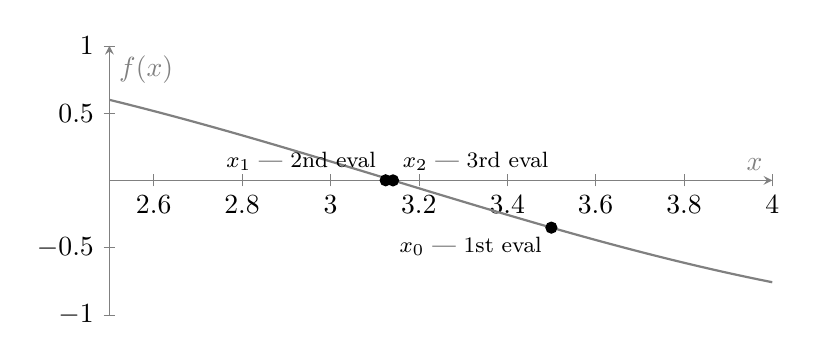
\begin{tikzpicture}
        \begin{axis}[
              width=10cm,
              height=5cm,
              axis x line=middle,
              axis y line=middle,
              xlabel={$x$},
              ylabel={$f(x)$},
              domain=2.5:4,
              samples=100,
              ymin=-1, ymax=1,
              xmin=2.5, xmax=4,
              legend style={at={(0.5,-0.2)},anchor=north},
              tick style={gray},
              label style={gray},
              axis line style={gray},
        ]
            % Continuous curve
        \addplot[gray, thick, smooth] {sin(deg(x))};
        % Newton iteration points
        \addplot[black, only marks, mark=*] coordinates {
            (3.5, -0.351)
            (3.125, 0.0008)
            (3.14159, 0.0)
        };
        % Iteration annotations
        \node[below left, font=\footnotesize] at (axis cs:3.5, -0.351) {$x_0$ | 1st eval};
        \node[above left, font=\footnotesize] at (axis cs:3.125, 0.0008) {$x_1$ | 2nd eval};
        \node[above right, font=\footnotesize] at (axis cs:3.14159, 0.0) {$x_2$ | 3rd eval};
        \end{axis}
    \end{tikzpicture}
    \caption{Newton's method iterations: starting from $x_0=3.5$, converging rapidly to $\pi \approx 3.14159$.}
    \label{fig:newton_sine_iteration}
\end{figure}

\marginnote{\newthought{We pay for this sophistication} with more hyperparameters that we need to determine and more 
complex computations (derivative evaluation and division), but we gain in convergence speed.}


\newthought{Derivative as source of local information} $f'(x) = \cos(x)$ 
gives the slope of the tangent at a given point. 
There are multiple ways to use this information to derive the direction and the size of the next step: We for sure want to move in the direction where the function decreases, then we could take a step with fixed size, or we could make the step size proportional to the derivative.
Let's just take the next guess where the tangent crosses zero for now - which is the solution to the linear approximation of $f$ at $x_n$. 


Starting at $x_0 = 3.5$:
\begin{align*}
    x_1 &= x_0 - \frac{\sin(x_0)}{\cos(x_0)}\\
    &= 3.5 - \frac{-0.351}{-0.936} \\
    &= 3.5 - 0.375 \\
    &= 3.125 \\
    x_2 &= 3.125 - \frac{\sin(3.125)}{\cos(3.125)} \\
    &= 3.125 - \frac{0.0008}{-0.9999} \\
    &\approx 3.14159 \\
    x_3 &\approx 3.14159 \\
    \text{and } \sin(3.14159) &\approx 0
\end{align*}

After just 2 iterations, to be fair this means 4 function/derivative evaluations, we have $x \approx 3.14159$ with error $< 10^{-5}$.
The derivative told us where to look way more efficiently than we have been used to.


\vspace{2.5em}
\newthought{The Learning Objectives} of this chapter aim at providing you with the abilities to:
\begin{itemize}
    \item Derive and apply Newton-Raphson iteration for root finding in 1D
    \item Derive and understnad the Taylor expansion and its role in Newton's method
    \item Analyze convergence rates and failure modes for Newton's method
    \item Understand and apply the Secant method when derivatives are unavailable
\end{itemize}

\marginnote{\newthought{"Newton-Rhapson"} because Isaac Newton came up with the general idea, 
while Joseph Raphson simplified the approach into a practical iterative method.}



% ==============================================================================================
% MAIN THEORY BLOCK
\newpage
\section{Newton-Raphson and Taylor Expansion}
\index{Newton-Raphson}
\index{linear approximation}

\begin{figure}[h]
    \centering
    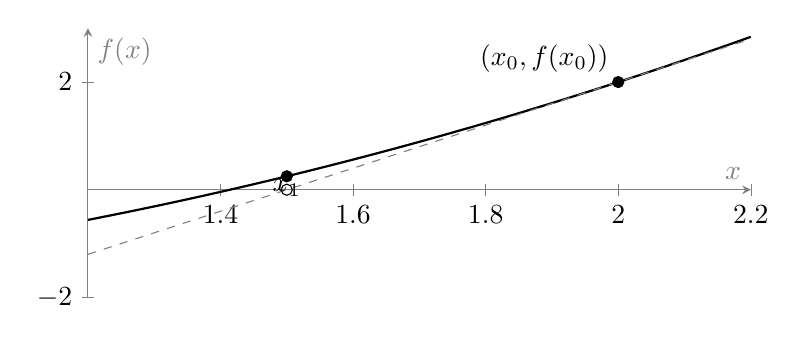
\begin{tikzpicture}
        \begin{axis}[
            width=10cm,
            height=5cm,
            axis x line=middle,
            axis y line=middle,
            xlabel={$x$},
            ylabel={$f(x)$},
            domain=1.2:2.2,
            samples=100,
            ymin=-2, ymax=3,
            xmin=1.2, xmax=2.2,
            tick style={gray},
            label style={gray},
            axis line style={gray},
        ]
        % The function f(x) = x^2 - 2
        \addplot[black, thick, smooth] {x^2 - 2};

        % Tangent line at x=2: f(2)=2, f'(2)=4, tangent: y-2=4(x-2) => y=4x-6
        \addplot[gray, dashed, domain=1.2:2.2] {4*x - 6};

        % Point at x_0 = 2
        \addplot[black, only marks, mark=*, mark size=2pt] coordinates {(2, 2)};
        \node[above left] at (axis cs:2,2) {$(x_0, f(x_0))$};

        % Point where tangent crosses x-axis: x = 1.5
        \addplot[black, only marks, mark=o, mark size=2pt] coordinates {(1.5, 0)};
        \node[above] at (axis cs:1.5,-0.3) {$x_1$};

        % Solid dot on curve at x = 1.5 and f(x)
        \addplot[black, only marks, mark=*, mark size=2pt] coordinates {(1.5, 0.25)};

        \end{axis}
    \end{tikzpicture}
    \caption{Newton's method geometric intuition: For $f(x) = x^2 - 2$, the tangent line at $(x_0, f(x_0))$ intersects the $x$-axis at $x_1$, our next approximation.}
    \label{fig:newton_geometric}
\end{figure}

\vspace{1em}

\newthought{Above} you can see the geometric intuition behind Newton's method for a single iteration. 
Let's formalize the approach of finding $x^*$ such that $f(x^*) = 0$.

\marginnote{\newthought{Note:} This linear approximation is the first-order Taylor expansion of $f$ around $x_n$. We'll return to Taylor expansions later when we study accuracy and approximation formally.}

\newthought{The linear approximation is effectively} given as:
\begin{equation}
    f(x) \approx  f'(x_n) \cdot (x - x_n) \quad \text{for } x \text{ close to } x_n + f(x_n)
\end{equation}

\newthought{Finding the next guess:} We want to find where this linear approximation crosses zero, 
because this is our best guess for where the actual function crosses zero. Setting the approximation to zero:

\begin{align*}
    0 &= f(x_n) + f'(x_n) \cdot (x_{n+1} - x_n) \\
    f'(x_n) \cdot (x_{n+1} - x_n) &= -f(x_n) \\
    x_{n+1} - x_n &= -\frac{f(x_n)}{f'(x_n)}
\end{align*}

This gives us the Newton-Raphson iteration formula:
\begin{equation}
    x_{n+1} = x_n - \frac{f(x_n)}{f'(x_n)}
\end{equation}


\vspace{1.5em}
\begin{algorithm}[H]
\caption{Newton-Raphson Method}
\begin{algorithmic}[1]
    \Require Initial guess $x_0$, function $f$, derivative $f'$, tolerance $\varepsilon$
    \State $x \gets x_0$
    \While{$|f(x)| > \varepsilon$}
        \State Compute derivative: $d \gets f'(x)$
        \If{$|d| < \varepsilon_{\text{machine}}$}
            \State \textbf{error} ``Derivative too small''
        \EndIf
        \State Update: $x \gets x - f(x) / d$
    \EndWhile
    \Return $x$
\end{algorithmic}
\end{algorithm}
\marginnote{\newthought{This error} occurs when the derivative $f'(x_k)$ approaches zero, 
which would cause division by zero or numerical instability in Newton's method.}






\section{Taylor Expansion}
\index{Taylor expansion}

\newthought{So far we did just trust} the linear approximation at $x_n$:

\begin{align}
    f(x) \approx f'(x_n)(x - x_n) + f(x_n),
\end{align}

to quickly find the next guess $x_{n+1}$ and finally converge to the root, but is that trust well placed?\\

The answer lies in the Taylor expansion, a fundamental tool that tells us how well 
polynomials approximate smooth functions at a given point.

\marginnote{\newthought{Smooth: } A function is smooth if it has derivatives of all orders, 
and is thus differentiable} 

Let's derive it from first principles to understand why the linear approximation is a good choice 
for Newton's method, 
and how we can systematically improve it if needed. 
To illustrate let's approximate the sine function step by step.

\begin{figure}[h]
    \centering
    % Requires: \usepackage{pgfplots}
    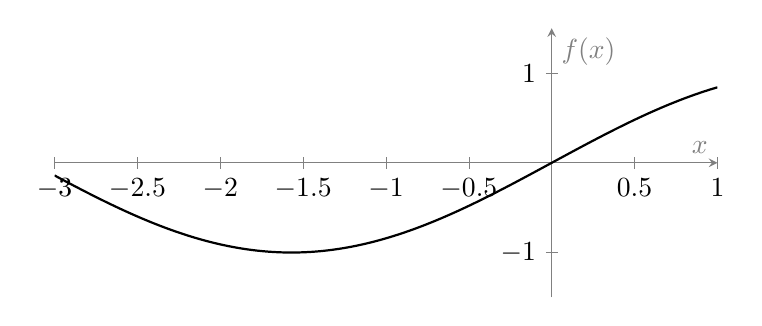
\begin{tikzpicture}
        \begin{axis}[
              width=10cm,
              height=5cm,
              axis x line=middle,
              axis y line=middle,
              xlabel={$x$},
              ylabel={$f(x)$},
              domain=-3:1,
              samples=100,
              ymin=-1.5, ymax=1.5,
              xmin=-3, xmax=1,
              legend style={at={(0.5,-0.2)},anchor=north},
              tick style={gray},
              label style={gray},
              axis line style={gray},
        ]
        % Continuous curve
        \addplot[black, thick, smooth] {sin(deg(x))};
        % Discretized points
        \end{axis}
    \end{tikzpicture}
    \caption{Continuous curve $f(x) = \sin(x)$ and its discretized version (black dots) on $[-3,1]$ with step size $h=1$.}
    \label{fig:sine}
\end{figure}


\newthought{0th Order: Match the function value.} 
We want a polynomial $P(x)$ that approximates $f(x)$ near $x_n$. Start with matching at the point itself:
\begin{equation}
    P(x_n) = f(x_n)
\end{equation}

This comes very close to what grid search does: it only looks at the function value at discrete points, without any information about how the function behaves between those points.

\begin{figure}[h]
    \centering
    % Requires: \usepackage{pgfplots}
    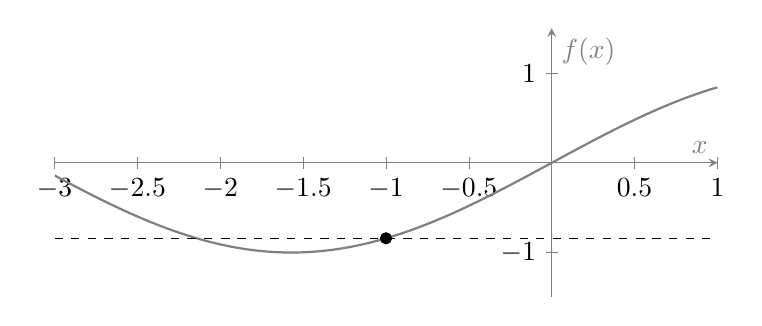
\begin{tikzpicture}
        \begin{axis}[
              width=10cm,
              height=5cm,
              axis x line=middle,
              axis y line=middle,
              xlabel={$x$},
              ylabel={$f(x)$},
              domain=-3:1,
              samples=100,
              ymin=-1.5, ymax=1.5,
              xmin=-3, xmax=1,
              legend style={at={(0.5,-0.2)},anchor=north},
              tick style={gray},
              label style={gray},
              axis line style={gray},
        ]
        % Continuous curve
        \addplot[gray, thick, smooth] {sin(deg(x))};
        % Horizontal approximation at x=-1.5
        \addplot[black, dashed, domain=-3:1] {sin(deg(-1))};
        % Mark the point at x=-1
        \addplot[black, only marks, mark=*, mark size=2pt] coordinates {(-1, {sin(deg(-1))})};
        \end{axis}
    \end{tikzpicture}
    \caption{Continuous curve $f(x) = \sin(x)$ with constant approximation $P(x) = f(-1)$ (black dashed line) anchored at $x=-1$ (black dot).}
    \label{fig:sine_constant_approx}
\end{figure}




\newthought{1st Order: Match the first derivative.}
Near $x_n$, the function's slope matters. We want $P'(x_n) = f'(x_n)$.

Adding a linear term:
\begin{equation}
    P(x) = f(x_n) + f'(x_n)(x - x_n)
\end{equation}

\begin{figure}[h]
    \centering
    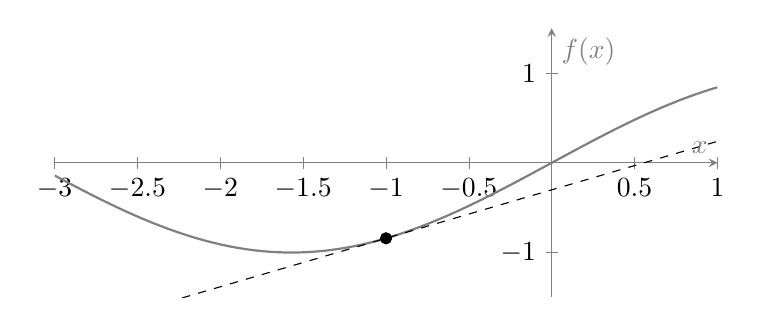
\begin{tikzpicture}
        \begin{axis}[
              width=10cm,
              height=5cm,
              axis x line=middle,
              axis y line=middle,
              xlabel={$x$},
              ylabel={$f(x)$},
              domain=-3:1,
              samples=100,
              ymin=-1.5, ymax=1.5,
              xmin=-3, xmax=1,
              legend style={at={(0.5,-0.2)},anchor=north},
              tick style={gray},
              label style={gray},
              axis line style={gray},
        ]
        % Continuous curve
        \addplot[gray, thick, smooth] {sin(deg(x))};
        % Linear approximation: tangent line at x=-1
        % f(-1) = sin(-1) ≈ -0.8414, f'(-1) = cos(-1) ≈ 0.5403
        % P(x) = sin(-1) + cos(-1)*(x - (-1)) = -0.8414 + 0.5403*(x+1)
        \addplot[black, dashed, domain=-3:1] {sin(deg(-1)) + cos(deg(-1))*(x+1)};
        % Mark the point at x=-1
        \addplot[black, only marks, mark=*, mark size=2pt] coordinates {(-1, {sin(deg(-1))})};
        \end{axis}
    \end{tikzpicture}
    \caption{Continuous curve $f(x) = \sin(x)$ with linear approximation $P(x) = f(-1) + f'(-1)(x+1)$ (black dashed tangent line) anchored at $x=-1$ (black dot).}
    \label{fig:sine_linear_approx}
\end{figure}



\newthought{2nd Order: Match the second derivative.}
The curvature captures how the slope changes. We want $P''(x_n) = f''(x_n)$.
Adding a quadratic term:
\begin{equation}
    P(x) = f(x_n) + f'(x_n)(x - x_n) + \frac{f''(x_n)}{2}(x - x_n)^2
\end{equation}


\begin{figure}[h]
    \centering
    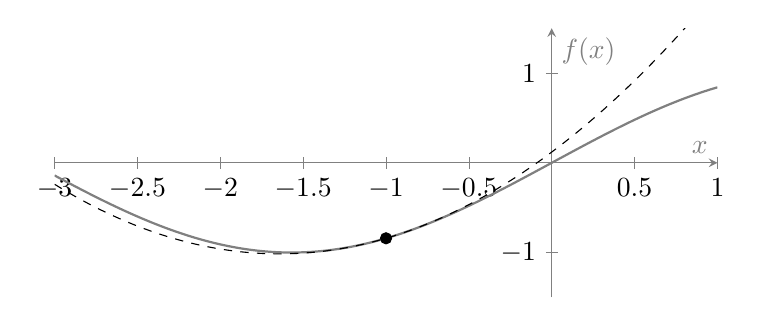
\begin{tikzpicture}
        \begin{axis}[
              width=10cm,
              height=5cm,
              axis x line=middle,
              axis y line=middle,
              xlabel={$x$},
              ylabel={$f(x)$},
              domain=-3:1,
              samples=100,
              ymin=-1.5, ymax=1.5,
              xmin=-3, xmax=1,
              legend style={at={(0.5,-0.2)},anchor=north},
              tick style={gray},
              label style={gray},
              axis line style={gray},
        ]
        % Continuous curve
        \addplot[gray, thick, smooth] {sin(deg(x))};
        % Quadratic approximation: Taylor expansion at x=-1
        % f(-1) = sin(-1) ≈ -0.8414, f'(-1) = cos(-1) ≈ 0.5403, f''(-1) = -sin(-1) ≈ 0.8414
        % P(x) = sin(-1) + cos(-1)*(x+1) + (-sin(-1))/2*(x+1)^2
        \addplot[black, dashed, domain=-3:1] {sin(deg(-1)) + cos(deg(-1))*(x+1) + (-sin(deg(-1)))/2*(x+1)^2};
        % Mark the point at x=-1
        \addplot[black, only marks, mark=*, mark size=2pt] coordinates {(-1, {sin(deg(-1))})};
        \end{axis}
    \end{tikzpicture}
    \caption{Continuous curve $f(x) = \sin(x)$ with quadratic approximation $P(x) = f(-1) + f'(-1)(x+1) + \frac{f''(-1)}{2}(x+1)^2$ (black dashed parabola) anchored at $x=-1$ (black dot).}
    \label{fig:sine_quadratic_approx}
\end{figure}



\marginnote{\newthought{Why divide by 2?} When we differentiate $(x-x_n)^2$ twice, we get 2. 
So if we want $P''(x_n) = f''(x_n)$, we need to divide by 2 to cancel this factor.}




\newthought{nth Order: General pattern.}

\newthought{The Taylor expansion} of a function $f$ around a point $x_n$ is given by:
\begin{equation*}
    f(x) = f(x_n) + f'(x_n)(x - x_n) + \frac{f''(x_n)}{2!}(x - x_n)^2 + \frac{f'''(x_n)}{3!}(x - x_n)^3 + \cdots
\end{equation*}

Or more compactly:
\begin{equation}
    f(x) = \sum_{k=0}^{\infty} \frac{f^{(k)}(x_n)}{k!}(x - x_n)^k
\end{equation}



\marginnote{\newthought{Around a point.} Visually we can see that the approximations are anchored on a specific point $x_n$. 
The Taylor expansion is a local approximation.}



\newthought{Why linear is enough for Newton?} \\
We want to solve $f(x^*) = 0$, not compute $f(x)$ as best as we can.
Improving an approximation of course comes with a cost: We need to compute higher derivatives 
and evaluate more complex polynomials.
In numerical computations we always need to decide where to cut off the Taylor series. 
We do so at some finite order, and the linear term is the first non-constant term that 
gives us directional information.

\index{quadratic convergence}

\newthought{Deriving the convergence rate}. Recall from Chapter 3, that a method is convergent if our approximation reaches a specific stable limit. 
For Newton's method finding a root $x^*$ where $f(x^*) = 0$, we want:
\begin{equation}
    |x_n - x^*| \to 0 \quad \text{as } n \to \infty
\end{equation}

Thanks to the Taylor expansion, we can quantify how fast the error decreases.\\

Let $e_n = x_n - x^*$ be the error at iteration $n$. 
Applying a 2nd Order Taylor expansion to $f$ around the true root $x^*$:
\begin{equation}
    f(x_n) = f(x^*) + f'(x^*)(x_n - x^*) + \frac{f''(\xi)}{2}(x_n - x^*)^2,
\end{equation}

where $\xi$ is some point between $x_n$ and $x^*$. Since $f(x^*) = 0$, this simplifies to:
\begin{equation}
    f(x_n) = f'(x^*) \cdot e_n + \frac{f''(\xi)}{2} e_n^2
\end{equation}
Where $e_n = x_n - x^*$ is the error at iteration $n$.

\newthought{Now apply Newton's formula:}
\begin{align*}
    e_{n+1} &= x_{n+1} - x^* \\
    &= x_n - \frac{f(x_n)}{f'(x_n)} - x^* \\
    &= (x_n - x^*) - \frac{f(x_n)}{f'(x_n)} \\
    &= e_n - \frac{f(x_n)}{f'(x_n)}
\end{align*}

and substitute the simplified Taylor expansion for $f(x_n)$:
\begin{equation}
    e_{n+1} = e_n - \frac{f'(x^*) \cdot e_n + \frac{f''(\xi)}{2} e_n^2}{f'(x_n)}.
\end{equation}

\newthought{For points close to $x^*$,}  we can make the assumption that $f'(x_n) \approx f'(x^*)$,

\marginnote{\newthought{Notice the assumption play out:} $10^{-1} \to 10^{-2} \to 10^{-3} \to 10^{-6} \to 10^{-12}$.
Once we're close enough and our assumptions hold (after iteration 2), the error squares perfectly, demonstrating quadratic convergence.}


\begin{equation}
    e_{n+1} \approx e_n - \frac{f'(x^*) \cdot e_n + \frac{f''(\xi)}{2} e_n^2}{f'(x^*)} = e_n - e_n - \frac{f''(\xi)}{2f'(x^*)} e_n^2
\end{equation}

which makes the first order error term cancel out, leaving us with:

\begin{equation}
    e_{n+1} \approx -\frac{f''(\xi)}{2f'(x^*)} e_n^2
\end{equation}

\newthought{In more abstract terms,} we can write this as:
\begin{equation}
    |e_{n+1}| \leq C \cdot |e_n|^2
\end{equation}
Which means that the error at the next iteration is approximately proportional to the square of the current error, where $C$ is a constant that depends on the function's curvature and slope at the root.

\newthought{This is quadratic convergence.} 

\vspace{1.5em}
Let's come back to our introductory example of computing $\sqrt{2}$ with Newton starting from $x_0 = 2$:

\begin{table*}[h]
\centering
\begin{tabular}{p{0.25\textwidth}p{0.37\textwidth}p{0.38\textwidth}}
\toprule
\textbf{$n$} & \textbf{$x_n$} & \textbf{$|e_n|$ (error)} \\
\midrule
0 & 2.000000000 & $5.86 \times 10^{-1}$ \\
1 & 1.500000000 & $8.58 \times 10^{-2}$ \\
2 & 1.416666667 & $2.45 \times 10^{-3}$ \\
3 & 1.414215686 & $2.13 \times 10^{-6}$ \\
4 & 1.414213562 & $4.5 \times 10^{-12}$ \\
\bottomrule
\end{tabular}
\vspace{2em}
\caption{Newton's method for computing $\sqrt{2}$. See how the error approximately squares each iteration.}
\label{tab:newton_sqrt2}
\end{table*}



\index{Newton failure modes}
\newthought{Newton's method can fail} in several ways, which we will endure for now, 
and for which we will find solutions later on. As a brain teaser, it is a nice exercise to 
visualize the failure modes in this plot: 

\begin{figure}[h]
    \centering
    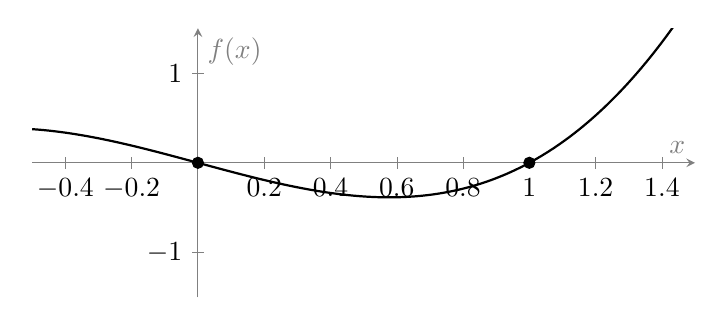
\begin{tikzpicture}
        \begin{axis}[
            width=10cm,
            height=5cm,
            axis x line=middle,
            axis y line=middle,
            xlabel={$x$},
            ylabel={$f(x)$},
            domain=-0.5:1.5,
            samples=100,
            ymin=-1.5, ymax=1.5,
            xmin=-0.5, xmax=1.5,
            tick style={gray},
            label style={gray},
            axis line style={gray},
        ]
        % f(x) = x^3 - x (has roots at -1, 0, 1)
        \addplot[black, thick, smooth] {x^3 - x};
        % Mark the roots (only 0 and 1 are in the visible range)
        \addplot[black, only marks, mark=*, mark size=2pt] coordinates {(0, 0) (1, 0)};
        \end{axis}
    \end{tikzpicture}
    \caption{$f(x) = x^3 - x$ has multiple roots. Newton's method can fail in several ways: 
    zero derivative (if $f'(x_n) = 0$, the tangent is horizontal and doesn't cross the axis), 
    oscillation (especially for symmetrical functions Newton can cycle between points), 
    and ambiguous starting point selection ($x_0$, heavily influences which root is found).}
    \label{fig:newton_multiple_roots}
\end{figure}






\vspace{1em}

\index{Secant method}

\newthought{Now something we can not endure}, is if we can't compute $f'(x)$.\\

\marginnote{\newthought{This can happen because:} 
\begin{itemize}
    \item The derivative is expensive to compute.
    \item The function is given as a black box (e.g., a simulation).
    \item The function isn't differentiable everywhere.
\end{itemize}}

\marginnote{\newthought{In deep learning,} we painstakingly make sure to design our loss functions, 
and activation functions to be differentiable, so that we we make sure that our gradients flow.}

\section{Secant Method}
Here comes a clever way to approximate the 
derivative using only function evaluations, eliminating the need for an explicit derivative.

\vspace{2em}
\newthought{A poor man's derivative.} Approximate the derivative using two recent points:
\begin{equation*}
    f'(x_n) \approx \frac{f(x_n) - f(x_{n-1})}{x_n - x_{n-1}}
\end{equation*}

\vspace{2em}
Visually this is the slope of the secant line connecting the points $(x_{n-1}, f(x_{n-1}))$ and $(x_n, f(x_n))$ on the graph of $f$:
\vspace{2em}
\begin{figure}[h]
    \centering
    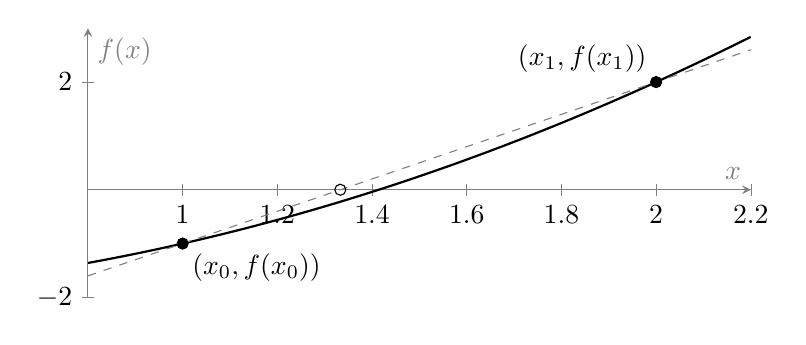
\begin{tikzpicture}
        \begin{axis}[
            width=10cm,
            height=5cm,
            axis x line=middle,
            axis y line=middle,
            xlabel={$x$},
            ylabel={$f(x)$},
            domain=0.8:2.2,
            samples=100,
            ymin=-2, ymax=3,
            xmin=0.8, xmax=2.2,
            tick style={gray},
            label style={gray},
            axis line style={gray},
        ]
        % The function f(x) = x^2 - 2
        \addplot[black, thick, smooth] {x^2 - 2};

        % Secant line through (1, -1) and (2, 2)
        \addplot[gray, dashed, domain=0.8:2.2] {3*x - 4};
        % Points
        \addplot[black, only marks, mark=*, mark size=2pt] coordinates {(1, -1) (2, 2)};
        \node[below right] at (axis cs:1,-1) {$(x_0, f(x_0))$};
        \node[above left] at (axis cs:2,2) {$(x_1, f(x_1))$};

        % Secant crosses at x = 4/3
        \addplot[black, only marks, mark=o, mark size=2pt] coordinates {(1.333, 0)};

        \end{axis}
    \end{tikzpicture}
    \caption{Secant method: the line through $(x_0, f(x_0))$ and $(x_1, f(x_1))$ gives the next approximation $x_2$.}
    \label{fig:secant_method}
\end{figure}

\vspace{2em}
\newthought{Note,} that this also means that we need two initial guesses $x_0$ and $x_1$ to start the iteration,
instead of just one for Newton's method.

Substituting into Newton's formula, gives us the iterative Secant method:
\begin{equation}
    x_{n+1} = x_n - f(x_n) \cdot \frac{x_n - x_{n-1}}{f(x_n) - f(x_{n-1})}
\end{equation}

\vspace{2em}
\newthought{And here's the algorithmic version formulated as a loop:}

\begin{algorithm}[H]
\caption{Secant Method}
\begin{algorithmic}[1]
    \Require Initial guesses $x_0$, $x_1$, function $f$, tolerance $\varepsilon$
    \While{$|f(x_1)| > \varepsilon$}
        \State Compute secant slope: $s \gets (f(x_1) - f(x_0)) / (x_1 - x_0)$
        \State Store previous: $x_{\text{old}} \gets x_1$
        \State Update: $x_1 \gets x_1 - f(x_1) / s$
        \State $x_0 \gets x_{\text{old}}$
    \EndWhile
    \Return $x_1$
\end{algorithmic}
\end{algorithm}




















% ==============================================================================================
% STUDENT ACTIVATION BLOCK

\newpage
\section{Examples \& Exercises}


\begin{figure}[h]
    \centering
    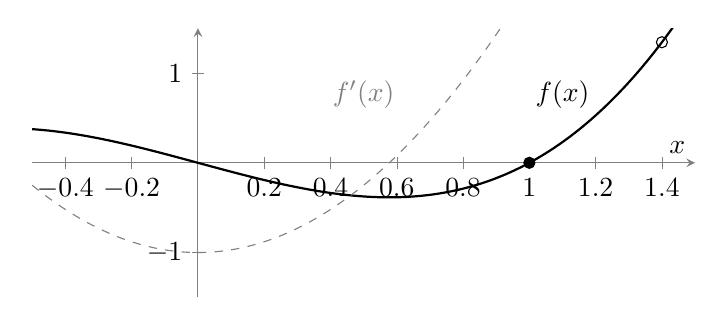
\begin{tikzpicture}
        \begin{axis}[
            width=10cm,
            height=5cm,
            axis x line=middle,
            axis y line=middle,
            xlabel={$x$},
            domain=-0.5:1.5,
            samples=100,
            ymin=-1.5, ymax=1.5,
            xmin=-0.5, xmax=1.5,
            tick style={gray},
            label style={black},
            axis line style={gray},
        ]
        % f(x) = x^3 - x (has roots at -1, 0, 1)
        \addplot[black, thick, smooth] {x^3 - x};
        % label for the function
        \node[above, black] at (axis cs:1.1,0.5) {$f(x)$};
        % Derivative f'(x) = 3x^2 - 1
        \addplot[gray, dashed, smooth] {3*x^2 - 1};
        % label for the derivative
        \node[above, gray] at (axis cs:0.5,0.5) {$f'(x)$};
        % Mark the roots (only 0 and 1 are in the visible range)
        \addplot[black, only marks, mark=*, mark size=2pt] coordinates {(1, 0)};
        % add a o mark at x=1.4 on the curve for x_0
        \addplot[black, only marks, mark=o, mark size=2pt] coordinates {(1.4, {1.4^3 - 1.4})};
        \end{axis}
    \end{tikzpicture}
    \caption{$f(x) = x^3 - x$ has multiple roots. We assume the root at $x = 1$ is the target. The gray dashed line shows the derivative $f'(x) = 3x^2 - 1$.}
    \label{fig:newton_excercises}
\end{figure}

\marginnote{\newthought{Code} can be found at \url{https://github.com/Quillstacks/lecturecode_numericalmethods.git}.}

\newthought{Newton by hand.} Find the root of $f(x) = x^3 - x = 0$ solving Newton's method geometrically, and then by hand.
The roots are at $x = -1, 0, 1$. Let's find the root at $x = 1$ starting from $x_0 = 1.4$. The 1st order Taylor expansion around $x_n$ gives us:
\begin{align*}
    f(x) \approx f(x_n) + f'(x_n)(x - x_n),\\
    f(x_n) \approx f(x) - f'(x_n)(x - x_n)
\end{align*}

We have $f(x) = x^3 - x = 0$, with  $f'(x) = 3x^2 - 1$, so we can rearrange to find the next guess,
starting from $x_0 = 1.4$:
\begin{align*}
    x_1 &= x_0 - \frac{f(x_0)}{f'(x_0)} \\
    &= x_0 - \frac{x_0^3 - x_0}{3x_0^2 - 1} \\
    &= 1.4 - \frac{2.744 - 1.4}{5.88 - 1} \\
    &= 1.4 - \frac{1.344}{4.88} \approx 1.127 \\
    x_2 &= 1.127 - \frac{1.127^3 - 1.127}{3(1.127)^2 - 1} \\
    &\approx 1.127 - \frac{0.432}{2.808} \\
    &\approx 0.976 \\
    x_3 &= 0.976 - \frac{0.976^3 - 0.976}{3(0.976)^2 - 1} \\
    &\approx 0.976 - \frac{-0.072}{1.857} \\
    &\approx 1.014
\end{align*}

The root at $x = 1$ is found quickly.


\newthought{Secant by hand.} Apply the Secant method to the same problem with $x_0 = 1.2$, $x_1 = 1.4$.
Again first geometrically, then by hand.

\begin{align*}
    x_2 &= x_1 - f(x_1) \cdot \frac{x_1 - x_0}{f(x_1) - f(x_0)} \\
    &= 1.4 - (0.744) \cdot \frac{1.4-1.2}{0.744 - 0.128} \\
    &= 1.4 - 0.744 \cdot \frac{0.2}{0.616} \\
    &\approx 1.4 - 0.241 \\
    &\approx 1.159 \\
    x_3 &= 1.159 - f(1.159) \cdot \frac{1.159 - 1.4}{f(1.159) - f(1.4)} \\
     &\approx 1.159 - (0.283) \cdot \frac{-0.241}{0.283 - 0.744} \\
     &\approx 1.159 - 0.283 \cdot \frac{-0.241}{-0.461} \\
     &\approx 1.159 - 0.283 \cdot 0.522 \\
     &\approx 1.159 - 0.148 \\
     &\approx 1.011
\end{align*}


\vspace{2em}
\newthought{Geometrical Failure Search.} 
Find starting points $x_0$ for different failure modes: One where Newton's method fails due to zero derivative, 
one where it converges to a non-target root, and one where it oscillates between points.


\newthought{Enter the machine.} Let's have a look on the convergence and convergence rates 
of Grid-Search, Newton and Secant method in Python. 
Then continue to experiment with differentstarting points, and observe the 
failure modes in practice. Try to first find the starting points geometrically, 
then try finding them analytically, 
before finally moving over to verifying in code.




\section{Self-Reflection and Recap}

\newthought{Self-Reflection} Questions to guide your understanding:
\begin{itemize}
    \item What is the main advantage of using Newton's method over Grid-Search?
    \item Why is a linear approximation sufficient for finding roots? What does the Taylor expansion tell us about this choice?
    \item Why is quadratic convergence so powerful? How many iterations would Newton need to go from error $10^{-1}$ to error $10^{-16}$?
    \item In what situations would you prefer Secant over Newton? Why not in others?
\end{itemize}

\newthought{Recap} of Key Concepts:
\begin{itemize}
    \item Newton-Raphson gives (limited) convergence guarantees near simple roots.
    \item Taylor expansion provides a systematic way to approximate functions locally.
    \item You saw how Taylor expansion justifies the linear approximation in Newton's method and explains its quadratic convergence and allows to estimate the error in each iteration.
    \item In situations where the derivative is difficult to compute, the Secant method approximates the derivative from two points and converges.
\end{itemize}


\marginnote{\newthought{Teaser.} How can we make sure that we find the global solution, and not just a local one?}

\newthought{Local methods find local solutions.} Newton converges to whatever optimum is nearby, 
it is also prone to oscillate between points, or diverge if the derivative is zero or near zero. In the next chapter, we will reformulate the root finding into an optimization problem.
And from there we'll explore how to go on and handle global optimization when the landscape has many valleys or is otherwise pathologically difficult.



%%%%%%%%%%%%%%%%%%%%%%%%%%%%%%%%%%%%%%%%%%%%%%%%%%%%%%%%%%%%%%%%%%%%%%%%%%%%%%
